\chapter{Structural boundary detection}
\label{Chap:MSA}
In popular Western music, songs typically consist of a sequence of \textit{segments}, named \textit{sections}, that are differently labeled depending on their role in the song, such as \textit{intro}, \textit{verse}, \textit{chorus}, \textit{bridge} and \textit{outro}, and that may appear multiple times in the same song. The structure is the higher hierarchical layer for the organization, composition and execution of a song. People commonly remember popular songs from a sample of their chorus or the bridge.%, and composers usually organize their songs as a sequence of sections, which are then easily memorized and executed by musicians.

Given the great importance of the musical structure for the organization of songs, the MIR community has devoted a great effort in the attempt of automatically extracting it from music signals. Automatic \textit{Musical Structural Analysis} (MSA) aims at identifying such sections and grouping them together, which are useful for numerous applications, such as the generation of audio summaries \cite{peeters2002toward} or the extraction of section-level descriptors for music retrieval purposes \cite{buccoli2015dimensional,chiarandini2011}.

MSA algorithms analyze songs with the purpose of automatically retrieving their structure. The semantic domain of the problem is well formalized, as discussed in Section \ref{sec:HLFs:MSA} since the structure is a musicological entity that has received in-depth studies. On the other side, the signal domain related to the problem is not fully understood, since many musical aspects might be involved. In order to design a proper audio representation for MSA, we need to assess which musical properties are relevant for segmentation purposes (e.g., timbre, harmony); and we need to design signal processing strategies to capture them. Traditionally, the signal domain is formalized as a feature-based representation of the audio signal (e.g., MFCCs, chromagram), which is usually hand-designed for that specific application. Since the semantic domain is clear, the linking function is usually modeled as a rule-based algorithm, as presented in Section \ref{sec:ML:MSA}.

It is difficult to find which properties are involved for musical structure analysis, and the designed features might not be able to capture the found properties. Moreover, structural analysis is a complex task that might involve other perceptual elements not captured by the designed features. Deep learning techniques offer an alternative to this approach, as they are able to automatically find an abstract representation of the musical content. In our work, we aim at evaluating the feasibility of learned features with respect to the hand-crafted features in the task of Music Structure Analysis. We specifically focus on the detection of the boundaries between sections, since this is a crucial task in MSA \cite{Nieto2D}. In order to asses the validity of our approach, we compare the learned representation of data with the most used hand-crafted features (chromagram and MFCC) by using some of the state-of-the-art MSA techniques presented in Section \ref{sec:ML:MSA}. This work was presented at the European Conference on Signal Processing (EUSIPCO) \cite{Buccoli2016MSA}.

The obtained boundaries define the semantically uniform sections of songs, but are also useful to formalize the signal domain. As an example, in Section \ref{sec:LLFs:hand-crafted} we mentioned the pooling techniques, that help to compute a compact representation from the frame-level representation, over fixed-length intervals, and the approach based on dynamic-length intervals given by the position of the beats of the song. The structural boundaries can also be used as long-time intervals for the pooling techniques, helping retrieving a representation of the signal domain that implicitly embeds semantic information. We might retrieve songs similar to a query example by only comparing the feature representation of the signal domain averaged over the sections. For this reason, while we model the automatic MSA as a linking function that computes the semantic domain from the signal domain, the retrieved information can be used to revert the direction and better formalize the signal domain. The structural boundaries can also enrich the semantic domain, as explained in Chapter \ref{Chap:HLFs}, to include the time-domain in the high-level description and obtain time-invariant semantic description.


 \begin{figure}[tb]
    \begin{center}
      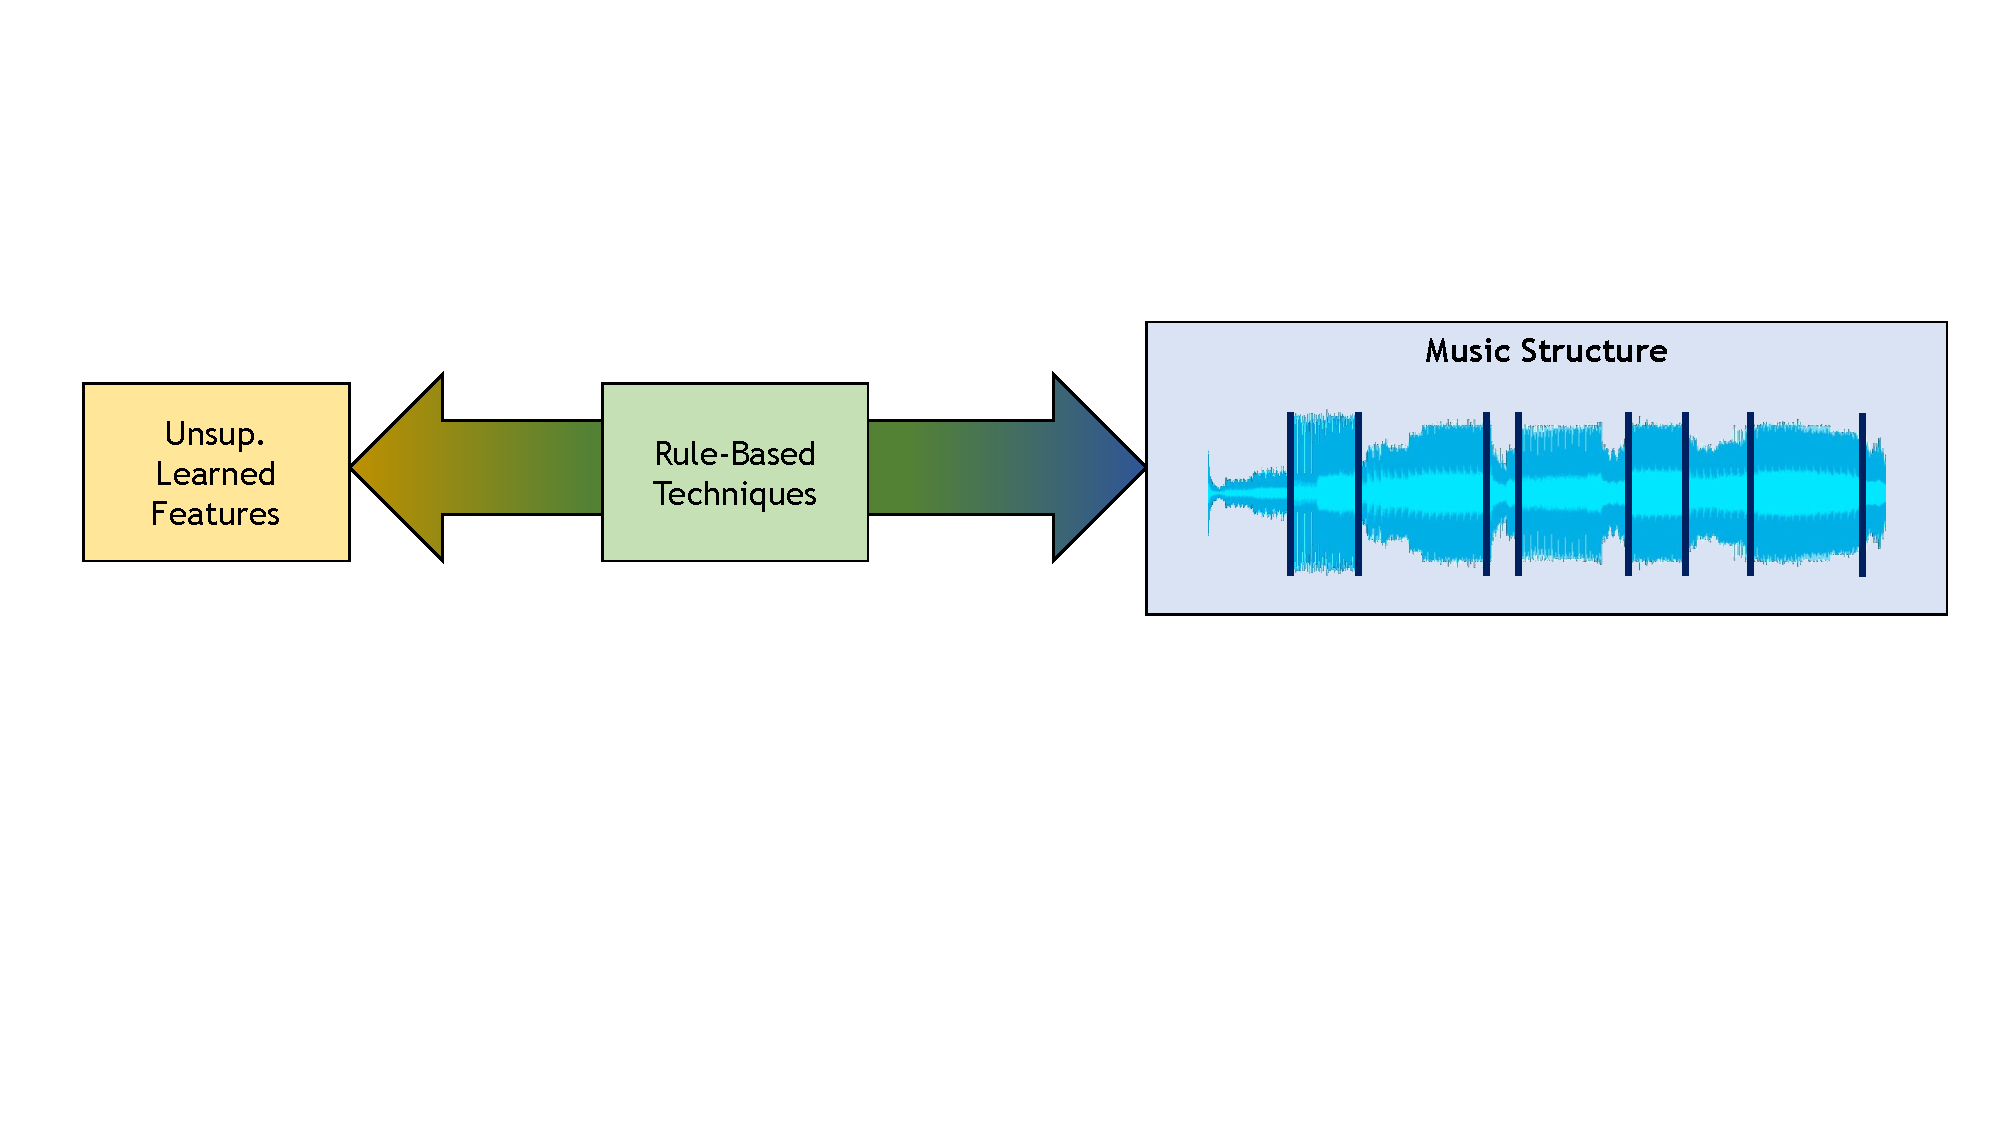
\includegraphics[trim=1.4cm 8.6cm 0.9cm 5cm,clip=true,width=\textwidth]{img/MSA/schema}
	%\psfig{file=im/ML/logopm.jpg,width=3.5cm}
    \end{center}
  \caption{The block diagram of the approach for the Music Structure Analysis proposed in this Chapter.}
  \label{fig:MSA:scheme}
  \end{figure}

In Figure \ref{fig:MSA:scheme} we show the block diagram visualization of the proposed approach for MSA, where we aim at retrieving the boundaries between sections by using rule-based techniques with unsupervised learned features. In the following Sections we provide an overview of the state of the art of Music Structure Analysis algorithm. We then explain how we collect the data for the formalization of the signal domain and the semantic domain. We evaluate our approach by using a set performance metrics from the literature on the automatic detection over a well-known annotated dataset for MSA and we draw some final considerations on this scenario. 

\section{Background}
\label{sec:MSA:intro}
MSA typically comprises two main steps: first the section boundaries are identified (\textit{boundary detection}); and then the related sections are clustered together in order to identify the structure of the song (\textit{clustering}). The aim of the clustering step is not to label the sections (i.e., it does not identify the role of the sections), but only to group similar sections in the same cluster. 
Since the codomain is well formalized, the MSA literature focuses on two main steps, the feature extraction and the segmentation techniques. In this Section, we provide an overview of the state of the art in this respect. 

\subsection{Features Extraction}
In \cite{bruderer2006structural}, the authors identify three main properties to which people give relevance when manually segmenting a song: the timbre, the harmony and the rhythm. The researchers have therefore focused on the extraction of features that capture such properties, as discussed in Section \ref{sec:LLFs:hand-crafted}.

The harmony is related and composed of the notes during the song, and therefore it is often captured by means of the chromagram \cite{NietoCNMF,Nieto2D,Jensen2007}, as a histogram of the distribution of the notes regardless of the octave. However, the chromagram descriptor is not robust to key-transposition within the songs which sometimes occur. In \cite{Nieto2D} a 2D Fourier Transform is used to achieve the invariance to key-transposition of the chromagram.

The timbre is usually captured by the MFCCs \cite{itoh2008automatic,cooper2002,dubnov2008unified}. More recently, the Gammatone filters have been used as an alternative  auditory system model to extract cepstral components or a metric of the contrast. Timbral features from Gammatone filters have been effectively employed for the MSA task by \cite{tian2016}.

The rhythm has received less attention by the community and only few works have explored the rhythmic-based features for the MSA. In \cite{Jensen2007} the author extract a representation called \textit{rhythmogram}, which computes the autocorrelation of a \textit{Perceptual Spectral Flux} (PSF), i.e., a note onset detector. The autocorrelation is able to spot the different repetitions of the notes at different periods, hence a measure of the rhythmic patterns. In \cite{Tian2015}, the authors extract a \textit{tempogram}, which is again the autocorrelation of an onset detection function, for the task of MSA.


\subsection{Automatic structure analysis}
The authors of \cite{paulus2010state} identify five main principles to compose or detect the structure of a song: the homogeneity, the contrast, the repetitions, the temporal order and the variations. The MSA literature summarizes these principles with two main approaches: the \textit{homogeneity-based}, or \textit{state-based}, and the \textit{repetition-based}, or \textit{sequence-based}. 

The state-based approach assumes that the musical content within a section is homogeneous (the homogeneity principle), and that the boundaries between two consecutive sections can be retrieved by identifying a discontinuity of such homogeneity (the contrast principle). This approach is usually implemented by analyzing some feature representation of the signal domain and defining a novelty curve that is able to spot such discontinuity in the feature representation. This approach is particularly effective when the acoustic properties of the songs do not significantly vary within sections \cite{kaiser2010music}. Several algorithms discussed in Section \ref{sec:ML:MSA} follow in fact this approach, such as the ones proposed by Foote \cite{foote2000automatic}, Serra et al. \cite{Serra2014}, Nieto et al. \cite{NietoCNMF} and Jensen \cite{Jensen2007}.

The sequence-based approach assumes that the musical content of two similar sections follows the same patterns (the repetition principle), with possible variations (the variation principle), and where the principle of temporal order is therefore crucial. The repetitions within a song are usually spotted by inspecting the self-similarity matrix (Section \ref{sec:ML:self}) computed from some feature-based representation of the signal domain, in order to retrieve diagonal stripes parallel to the main diagonal. The detection of such stripes is hard due to variations in dynamics and timbre or other musical factors \cite{muller2007towards,muller2007information}. The self-similarity matrix is therefore commonly processed in order to remove too short line stripes \cite{lu2004repeating,ong2007structural} and to reduce the noise \cite{bartsch2005audio,wellhausen2003audio,goto2003chorus}. Several techniques follow a sequence-based approach to extract the music structure: by using a probabilistic model and a Viterbi algorithm \cite{shiu2006similar}, pattern recognition techniques \cite{rhodes2007algorithms} or Hidden Markov Model for the transition within the patterns \cite{aucouturier2002finding}.
 
In the latest years, deep learning techniques have been used in a supervised fashion to perform boundary detection for MSA. In \cite{ullrich2014boundary}, the authors propose a Convolutional Neural Network (CNN) to extract a representation from some frames of the magnitude audio spectrum and directly compute the probability that a section boundary occurs among those frames. The same approach is refined with deeper architectures in \cite{grill2015music} and \cite{grill2015_ismir}. In this Chapter, instead, we only focus on the feature extraction stage, by using a merely unsupervised feature learning. 



\section{Formalization and collection of the signal domain and the semantic domain}\label{sec:MSA:domains}
We extract a set of learned features by means of a Deep Belief Network (DBN) (see Section \ref{sec:LLFs:learned}). We train a 3-layer DBN over a dataset $\Sdbn$, which is composed of 10,000 copyright-free, unlabeled songs from the Grand Challenge of User Experience (GCUX14) of MIREX\footnote{http://www.music-ir.org/mirex/wiki/2014:GC14UX}. 

Several representations of the audio content have been proposed for being used as input to the DBN, i.e., to define the vector $\mathbf{v}$ starting from the audio signal. Such proposed representations include the principal components of the spectrogram \cite{lee2009convolutional} or of the mel-scaled spectrum \cite{hamel2011}, or the magnitude of the spectrum \cite{Hamel2010}. We follow the latter procedure suggested in \cite{Hamel2010}, and we represent the input layer of the DBN as the standardized log-magnitude of the Fourier Transform of a frame-level representation of the audio files. More formally, we first down-sample the songs to 11025 Hz, since we experimentally assess that it does not effect the performance and save computational time. We divide each song $\mathbf{s}_i \in \Sdbn$ into a sequence of $F_i$ overlapping frames $\mathbf{s}_{i,f}, \; f\in\{1, ..., F_i\}$, with frames of 1024 samples and 50\% overlap, and we compute the set of the DBN training input $\mathcal{V}=\{\mathbf{v}_{i,f}\}$ as  
\begin{equation}
\mathbf{v}_{i,f} = \log_{10}(| \mathcal{F}(\mathbf{s}_{i,f}) |^2),
\end{equation}
where $\mathcal{F}$ represents the Fourier transform. In order to make data consistent, we standardize each frequency bin as explained in Section \ref{sec:ML:data}. We train the DBN in a layer-wise fashion and we obtain the network parameters  $\left\{\mathbf{\hat{W}}^{(k)},\mathbf{\hat{b}}^{(k)},\mathbf{\hat{c}}^{(k)} \right\}$ for each layer $k \in  \left\{1,2,3\right\}$ as discussed in Section \ref{sec:LLFs:learned}. We implement a 3-layer DBN, with 75, 50 and 25 neurons for the first, second and third layer, respectively. We train the DBN with a learning rate of $10^{-5}$ for $10$ epochs \cite{Bengio2009} for each layer. 

We use the network parameters to compute the learned features for unseen songs $s_{i} \notin \Sdbn$ for each layer and each frame of  $\mathbf{s}_{i,f}$ as: 
\begin{equation}
\mathbf{h}^{(k)}_{i,f} = \tau ( \hat{\mathbf{W}}^{(k)} \mathbf{h}^{(k-1)}_{i,f}+ \hat{\mathbf{c}}^{(k)}),
\end{equation}
where $\mathbf{h}^{(0)}_{i,f}=\mathbf{v}_{i,f}$. We compose the final feature vector $\mathbf{h}^{(ALL)}_{i,f}$ by stacking $\mathbf{h}^{(1)}_{i,f}$, $\mathbf{h}^{(2)}_{i,f}$ and $\mathbf{h}^{(3)}_{i,f}$ together.

Several musicology studies in the literature highlight that in popular Western music section boundaries  typically occur on the beat. For this reason, in order to make the method more robust to noisy fluctuations and independent from tempo variations, it is a common practice in MSA literature \cite{Nieto2D} to synchronize the feature extraction to the beat, as mentioned in Section \ref{sec:LLFs:hand-crafted}. We first automatically extract the beats and we then compute sequences of beat-synchronous feature vectors by averaging the feature vectors over the beat frames. %The beat-synchronization also makes the feature representation robust to tempo variation and the averaging over the beats help to smooth the representation and clean it from possible noise fluctuations. 

 \begin{figure}[t]
     \centering
     \subfloat[The SSM computed with hand-crafted and model-based features (MFCCs and chromagram).]{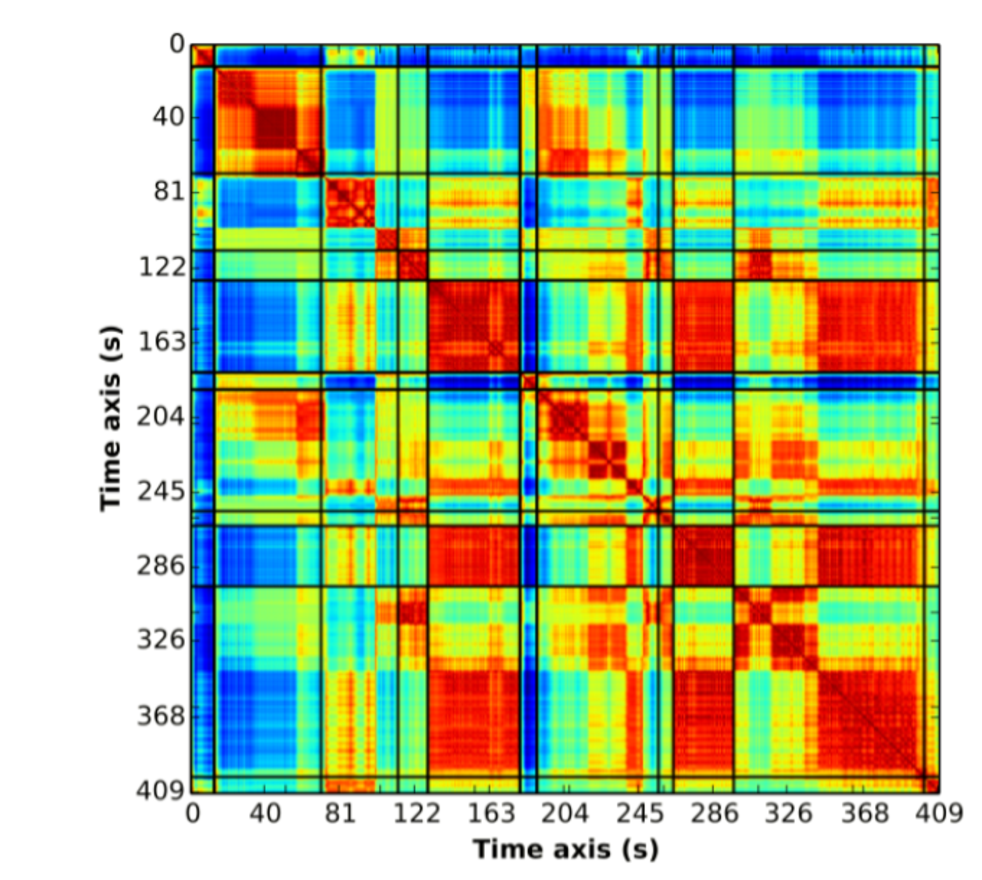
\includegraphics[width=.45\textwidth]{img/MSA/1008_hc_4}\label{fig:MSA:SSM_hc}} \hfil
    \subfloat[The SSM computed with learned features.]{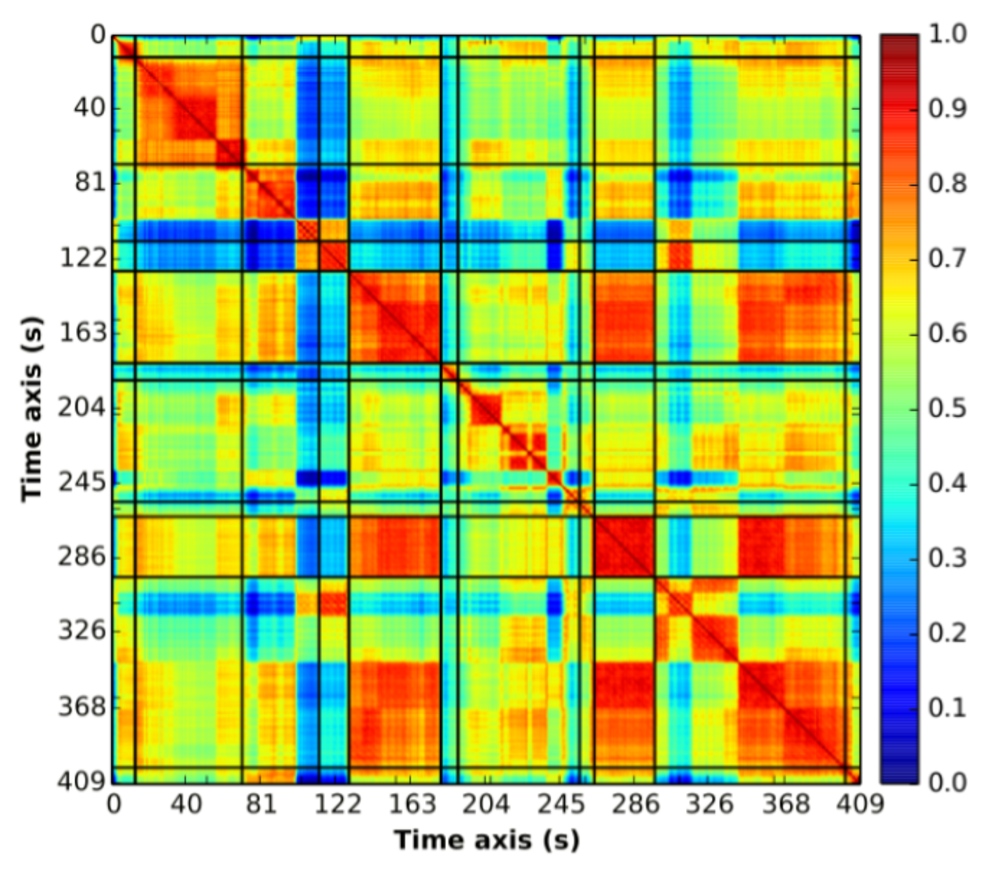
\includegraphics[width=.45\textwidth]{img/MSA/1008_dbn_4}\label{fig:MSA:SSM_dbn}}
     \caption{Comparison of the SSMs for the song \textit{Special Roll (6:59)} by Blacklite. The black lines indicate where the section boundaries occur.}
     \label{fig:MSA:SSM}
 \end{figure}
 
 
In this study we aim at comparing the learned feature representation with a traditional feature representation. For the comparison, we consider the two most commonly used hand-crafted or model-based features for MSA, i.e., the MFCCs and the chromagram, stacked together. In Figure \ref{fig:MSA:SSM} we show a comparison between two self-similarity matrices (SSMs) computed from hand-crafted (Fig. \ref{fig:MSA:SSM_hc}) and learned (Fig. \ref{fig:MSA:SSM_dbn}) features. The black lines indicate where the section boundaries occur. The best scenario for most of the MSA algorithms requires high and uniform self-similarity values in the blocks on the main diagonal and lower self-similarity values between contiguous blocks. We notice that the SSM generated from the learned features is visually neater. As an example, the self-similarity values of the section around 40s presents a noisy structure with the hand-crafted features, that may lead to over-segment that block, while with learned features is visually smoother, i.e., the values are more uniform within the block. For this reason, we expect that this might be a better representation for MSA.  

We formalize the semantic domain as discussed in Section \ref{sec:HLFs:MSA} using the function structure annotation, that identifies the semantic functions of the sections from a set of 20 labels. We used two annotated datasets to define the domain and evaluate the performance: a validation set $\SVALID$ composed of a set of $90$ songs by Queen, Michael Jackson and Carole King annotated by the Centre for Digital Music (C4DM) at Queen Mary, University of London\footnote{www.isophonics.net} and a test set $\STEST$, composed of $140$ freely-available songs of the so-called SALAMI Dataset \cite{Smith2011}. 

Given the set of $N=140$ songs $\STEST=\{s_1,...,s_N\}$, we formalize its boundary annotations as $\mathcal{Y}_{TEST}=\{y_1,...,y_N\}$, where each annotation $y_i$ with $i=1,...,N$ is composed by $B_i$ boundary instants:
\begin{equation}
y_i=\{b_1,...,b_{B_i}\}, 
\end{equation}
with $b_1=0s$ and $b_{B_i}$ equal to the duration of the song. 

\section{Experimental setup and evaluation}
\subsection{Experimental setup}
In order to evaluate our approach, we compare the performance of five techniques from the state of the art using hand-crafted and learned features:
\begin{enumerate}
\item \textit{Foote} correlates a Gaussian kernel along the main diagonal of the SSM to obtain a novelty curve from which peaks are extracted \cite{foote2000automatic};
\item \textit{C-NMF} is based on a decomposition of the SSM by using a convex non-negative matrix factorization \cite{NietoCNMF}; 
\item \textit{SF} is a repetition-based approach that uses structure features (SF) obtained from a time-lag matrix computed from a recurrence plot of the SSM \cite{Serra2014} ; 
\item \textit{SC} associates a recurrence plot of the SSM with a graph and applies spectral clustering (SC) techniques \cite{mcfee2014}; 
\item \textit{Jensen} retrieves boundaries as the shortest path of an adjacency matrix computed from the SSM \cite{Jensen2007}. 
\end{enumerate}
The algorithms were presented with a more extensive explanation in Section \ref{sec:ML:MSA}. These algorithms require to tune various parameters in order to improve the performance. For all the algorithms, we perform a grid search in the space of parameters in order to maximize the results over the validation set $\SVALID$. The algorithms are then executed again with the tuned parameters over the songs in $\STEST$. 
We choose to use the whole validation set instead of performing a cross-validation stage, in order to exploit the whole set of songs. Nevertheless, the two sets $\SVALID$ and $\STEST$ are completely disjoint in order to avoid overfitting issues. 

\begin{figure}[t]
\centering
\subfloat[Legend for the metrics on MSA]{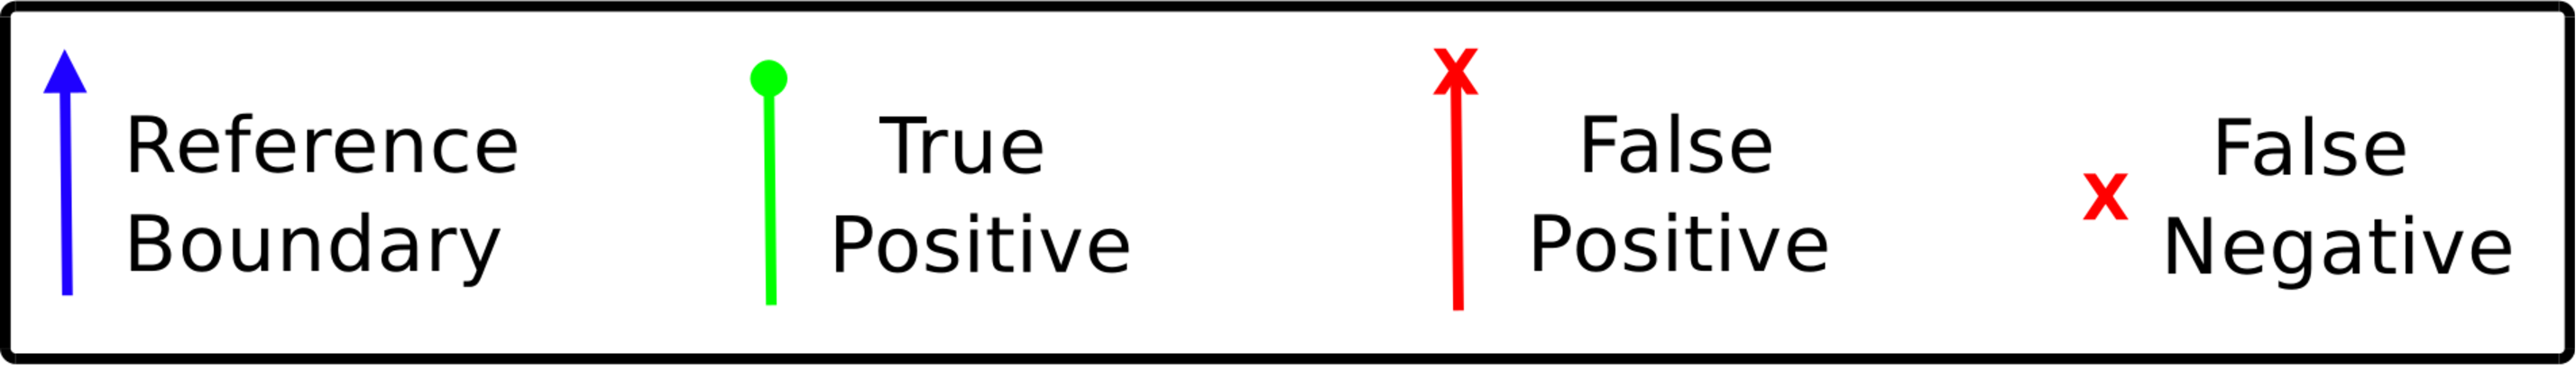
\includegraphics[width=.95\textwidth]{img/MSA/legend_metrics2}\label{fig:MSA:legend_metrics}} \hfil
\subfloat[Ground truth boundaries]{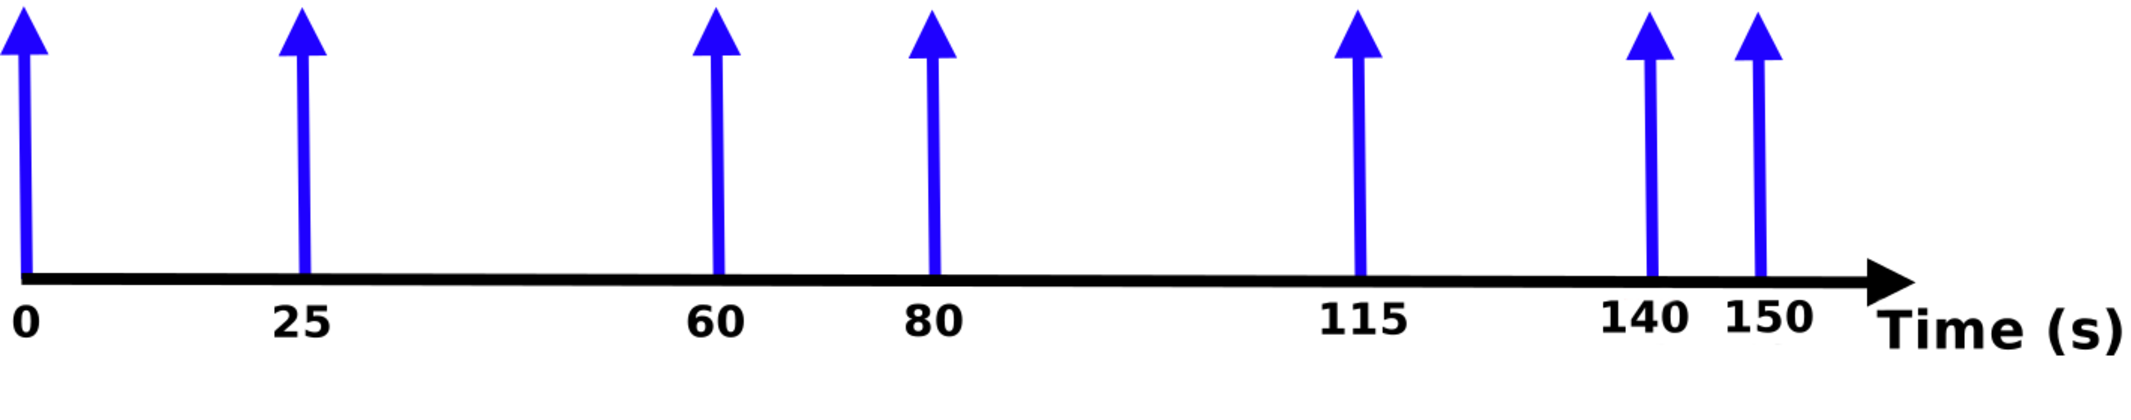
\includegraphics[width=.95\textwidth]{img/MSA/metrics2}\label{fig:MSA:expected_boundaries}} \hfil
\subfloat[Estimated boundaries]{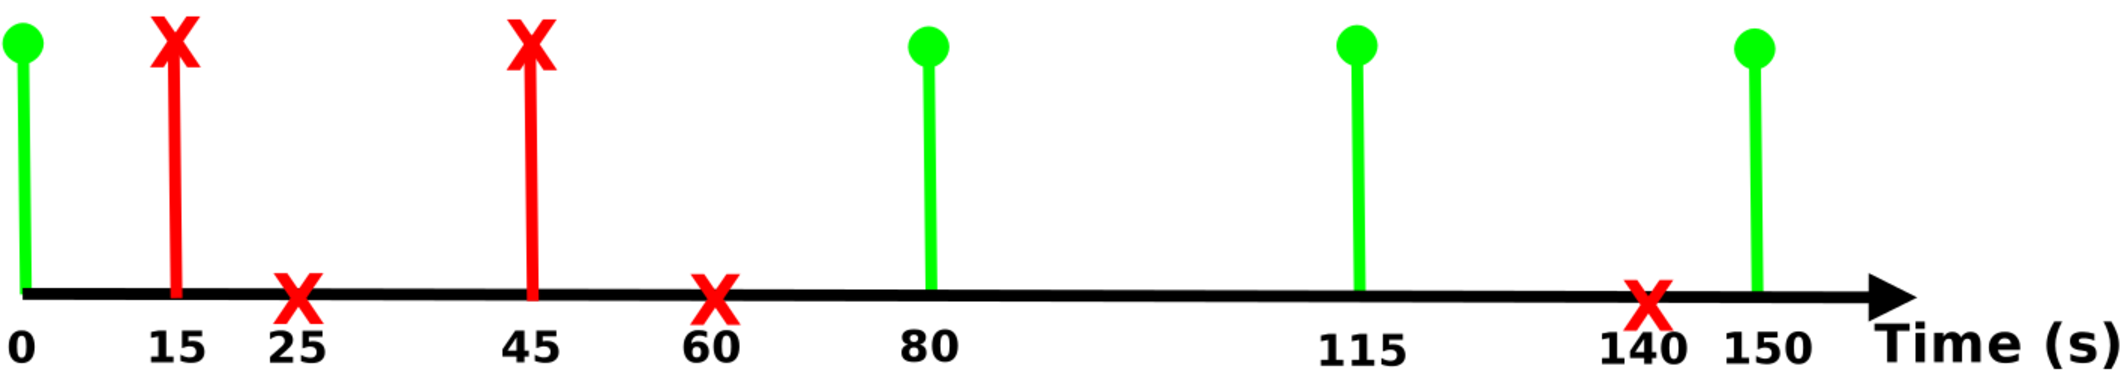
\includegraphics[width=.95\textwidth]{img/MSA/metrics_retrieved}\label{fig:MSA:estimated_boundaries}} 
\caption{A representation of the performance metrics for boundary detection}
\label{fig:MSA:boundaries_metrics}
\end{figure}

 
\subsection{Performance metrics}
In order to evaluate our approach, we considered the hit-measures Precision, Recall and F-measure, which are common metrics  in the literature and in the MIREX evaluation task. The Precision estimates the amount of correctly estimated boundaries, the Recall estimates the amount of correctly retrieved boundaries and the F-measure is a metric that summarizes the two above.

Given the generic annotated dataset $\mathcal{Y}$ as formalized in Section \ref{sec:MSA:domains}, the segmentation techniques aim at automatically detecting a set of boundaries:
\begin{equation}
\hat{y}_i=\{\hat{b}_1,...,\hat{b}_{\hat{B}_i}\},
\end{equation}
where the amount of detected boundaries $\hat{B}_i$ might be different from $B_i$ of the ground truth. The Precision, Recall and F-measure metrics estimate the similarity between the detected boundaries $\hat{y}_i$ and the ground-truth $y_i$.

Following the example in Figure \ref{fig:MSA:boundaries_metrics}, we first classify the estimated boundaries into three sets: True Positive ($TP$), False Positive ($FP$) and False Negative ($FN$). The positive boundaries are all those that have been correctly ($TP$) or incorrectly ($FP$) detected, while the false negative boundaries have not been detected. More formally:
\begin{equation}
TP=\{ \hat{b}_j \rightarrow \exists b_k: |b_k-\hat{b}_j|\leq \epsilon \};
\end{equation}
\begin{equation}
FP=\{ \hat{b}_j \rightarrow \nexists b_k: |b_k-\hat{b}_j|\leq \epsilon \};
\end{equation}
\begin{equation}
FN=\{ b_k  \rightarrow \nexists \hat{b}_j: |b_k-\hat{b}_j|\leq \epsilon \};
\end{equation}
where $\epsilon$ is the tolerance value. If a boundary is detected within the tolerance value from a boundary in the ground truth, it is marked as correctly estimated. Typical tolerance values, also used in the MIREX contest, are 0.5 and 3 seconds. The 3s tolerance value is more relaxed than the 0.5 seconds and usually more commonly used as a general evaluation of the algorithms, while the 0.5s tolerance is highly strict and even human annotators might fail to match it.

From $TP$, $FP$ and $FN$ we compute the Precision, the Recall and the F-measure metrics as in Equations \ref{eq:HLFs:P}, \ref{eq:HLFs:R} and \ref{eq:HLFs:F} respectively. The Precision ($P$) is the ratio of correctly detected boundaries over the total detected boundaries, while the Recall ($R$) is the ratio of correctly detected boundaries over the total annotated boundaries. In the following Section, we evaluate our approach by computing the average Precision, Recall and F-measure over all the song in $\STEST$ with 0.5 and 3 second tolerances.

\subsection{Numerical results}
 \begin{figure}[tb]
 	\centering
 	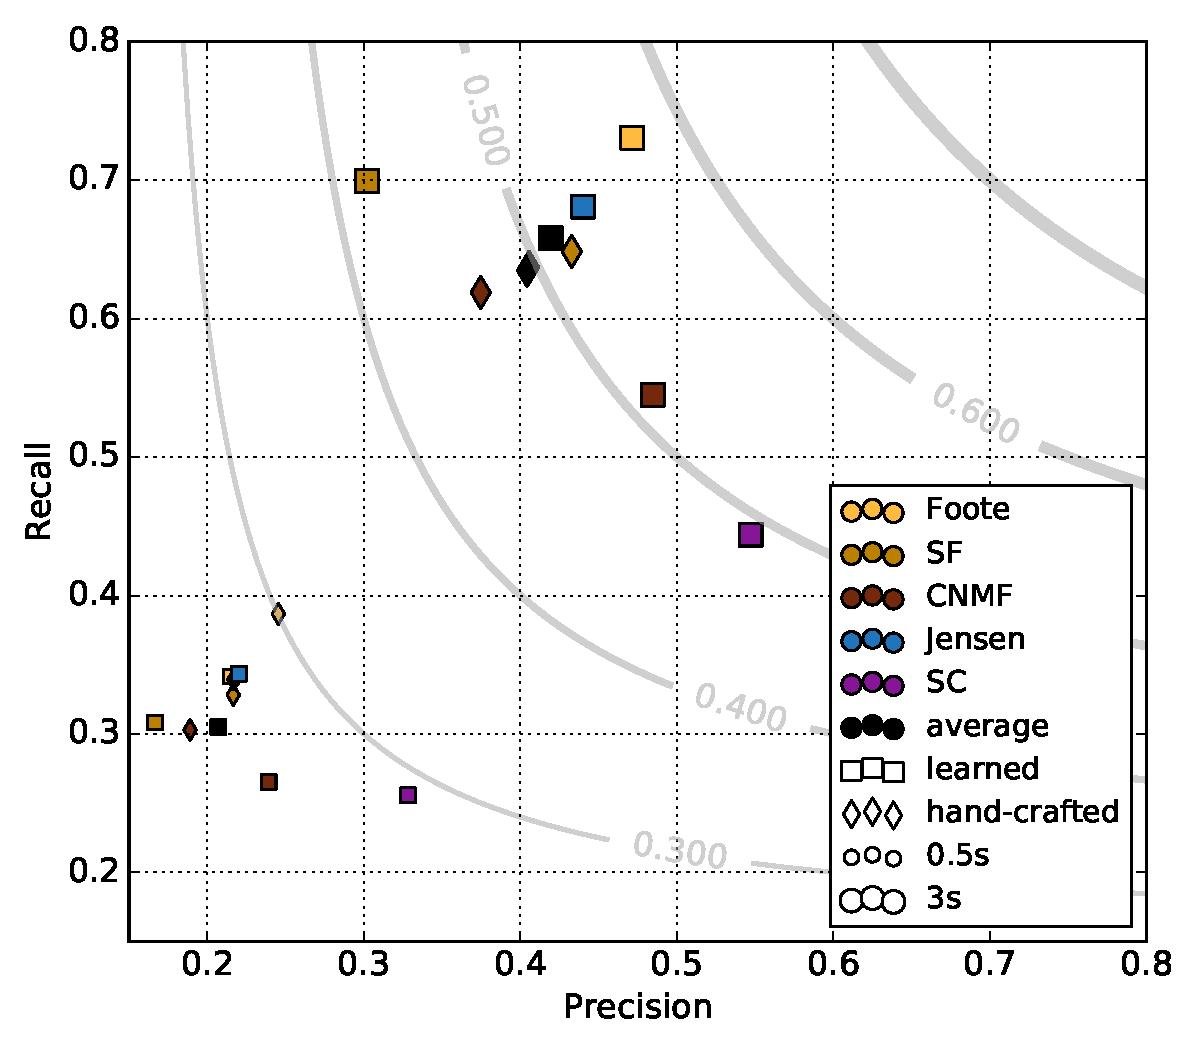
\includegraphics[width=.9\textwidth]{img/MSA/results_hc.pdf}
 	\caption{Scatterplot of the distribution of the results. The gray lines indicate the F-measure.}
     \label{fig:MSA:results}
 \end{figure} 

We perform the evaluation of our method over $\STEST$ by using the Python MIR evaluation framework\cite{mir_eval} and we compare the results with those published in the MIREX 2014 evaluation task in Structural Segmentation\footnote{{http://nema.lis.illinois.edu/nema\_out/mirex2014/results/struct/sal/}} for the same set of songs. We first provide the comparison of results between learned and hand-crafted features using Foote, SF and C-NMF algorithms and the average of such results, as shown in Table \ref{tab:MSA:results}. We then provide the results for the Jensen and SC algorithms, which are not part of the MIREX contest and for which we only show the results on the learned features in Table \ref{tab:MSA:resultsJSC}. The results in Tables \ref{tab:MSA:results} and \ref{tab:MSA:resultsJSC} are also graphically shown in a scatterplot in Figure \ref{fig:MSA:results}, where each marker is a different combination of algorithm (color of the market), feature (shape of the marker) and tolerance window (size of the marker). The gray lines in the scatter plot indicate different levels of F-measure.

From a visual inspection of the  Figure \ref{fig:MSA:results}, it is clear that, as mentioned, the 3-second tolerance value allows to achieve far higher results than the 0.5 second tolerance. The higher value of F-measure for the 0.5-second tolerance (F@0.5s) is achieved by an algorithm with hand-crafted features, and learned features are rather close to that result. The best performance for F@3s is achieved by an algorithm with learned features, as well as the higher P@3s and R@3s.

 \begin{table}[tb]
 \centering
 \caption{Precision, Recall and F-Measure (P, F, R respectively)  with 0.5 and 3 seconds of tolerance. The bold black font indicates which kind of features performs better for each algorithm.
 	Best and worst results over all the algorithms are in bold green and red italics fonts, respectively.}
 \label{tab:MSA:results}
%\large
 \bgroup
 \def\arraystretch{1.5}
 \begin{tabular}{||l|l|lll|lll||}
 \hline
  \hline
 %$\STEST$ 
 Algorithm & Feature    & P@0.5s    & R@0.5s    & F@0.5s     & P@3s     & R@3s     & F@3s   \\
 \hline
  \hline
 Foote & learned         & 0.2153 & 0.3415 & 0.2542 & 0.4715 & 0.7306 & {\color[HTML]{326B00}\textbf{0.5530} } \\
 Foote  & hand-crafted & 0.2454 & 0.3867 & {\color[HTML]{326B00} \textbf{0.2874}} & 0.4055 & 0.6371 & 0.4740  \\
\hline
 SF        & learned         & 0.1665 & 0.3083 & 
{\color[HTML]{8E0000} \textit{0.2067}} & 0.3021 & 0.6996 & 0.4741 \\
SF & hand-crafted & 0.2166 & 0.3282 & \textbf{0.2515} & 0.4328 & 0.6485 & 
% {\color[HTML]{326B00} 
\textbf{0.5013} \\
 \hline
CNMF      & learned         & 0.2392 & 0.2653 & \textbf{0.2421} & 0.4846 & 0.5451 & \textbf{0.4937} \\
CNMF & hand-crafted & 0.1890 & 0.3029 & 0.2230 & 0.3747 & 0.6190 & 
{\color[HTML]{8E0000} \textit{0.4470}} \\
\hline
average      & learned         &  0.2070 &  0.3050&  0.2343 &  0.4194    & 0.6584& \textbf{0.5070} \\
average & hand-crafted & 0.2170  &  0.3393&  \textbf{0.2540} &  0.4043& 0.6349& 0.4741  \\
         \hline
         \hline
 \end{tabular}
 \egroup
 \end{table}

As far as the Foote algorithm is concerned, the learned features perform slightly worse considering the F@0.5s, while they clearly outperform the hand-crafted features for F@3s. In particular, the performance exhibits a higher recall than precision, which leads us to suppose that the Foote algorithm might introduce a certain degree of over-segmentation, hence to be too sensible to variation with both kind of descriptors. 

As far as the C-NMF is concerned, the learned features outperform the hand-crafted ones both in the case of 0.5s and 3s tolerance. Moreover, while with the hand-crafted features the recall is much higher than the precision, they are rather balanced with the learned features. This implies that the learned features are more robust to slight variation of harmony or timbre, which might mislead the boundary detection.

The SF algorithm performs better with the hand-crafted features. We suppose this is because SF is based on the analysis of the repetition of patterns, while learned features seem to perform better with homogeneity-based algorithms. However, even with hand-crafted features, the SF algorithm never achieves the best performance for any of the evaluation metrics.

 \begin{table}[tb]
 \centering
 \caption{Precision, Recall and F-Measure (P, F, R respectively)  with 0.5 and 3 seconds of tolerance for the Jensen and SC algorithm.}
 \label{tab:MSA:resultsJSC}
% \large
 \bgroup
 \def\arraystretch{1.5}
 \begin{tabular}{||l|l|lll|lll||}
 \hline
  \hline
 Algorithm & Feature    & P@0.5s    & R@0.5s    & F@0.5s     & P@3s     & R@3s     & F@3s   \\
 \hline
  \hline
  Jensen     & learned         & 0.2203 & 0.3435 & 0.2559 & 0.4401 & 0.6810 & 0.5111 \\
  SC        & learned          & 0.3282 & 0.2557 & 0.2658 & 0.5471 & 0.4440 & 0.4592 \\
  \hline
   \hline
 \end{tabular}
 \egroup
 \end{table}

The average results show that the learned features perform worse than hand-crafted features for the 0.5-second tolerance, and better for the 3-second tolerance. It is clear that learned features achieve far different results with the two tolerance values, due to the generic unsupervised training step. Indeed, in \cite{ullrich2014boundary} it is shown that the same parameters setup for a CNN achieves highly different performance for the two tolerance values. The authors perform an analysis over the parameters' space for their MSA algorithm for the two tolerance levels. Since we aim at finding a generic feature representation for several MSA algorithms from the state of the art and with all the tolerance values, we do not test different setups for the different tolerance values. The proposed setup, instead, achieves fairly high results for all the algorithms and all the tolerance levels.

We now analyze the SC and Jensen algorithm, that we test only with learned features. The SC algorithm obtains optimal performance with the tolerance of 0.5s, since it is able to outperform most of the algorithms, including the SF. However, it exhibits poor general performance on the 3s tolerance. On the other hand, the algorithm proposed by Jensen exhibits average results with the 0.5s tolerance, while it outperforms all the other algorithms in the 3s, except for the one by Foote in the case of learned features. 

We draw some overall considerations by inspecting again Figure \ref{fig:MSA:results}. The Foote algorithm achieves the best performance both with F@0.5s (hand-crafted features) and F@3s (learned features). This are also the best results for the Recall metric, i.e., the algorithm by Foote is particularly effective in retrieving boundaries. Moreover, its precision is also fairly high, which indicates that most of the retrieved boundaries are correct. When focusing on the Precision metrics, however, the SC algorithm is the best technique for both tolerance values using the learned features. In both cases, however, it also achieves the worst Recall metrics, which means that the algorithm is not retrieving enough boundaries, i.e., it is under-segmenting.

\section{Final considerations}
We explored the linking function between the signal domain and the semantic domain in the MSA task. %This case was simple, due to the well formalization of the MSA task. 
We relied on the semantic formalization of MSA, which allowed us to use rule-based techniques from the state of the art to model the linking function. However, since the properties involved in the signal domain were not enough clear, we employed a deep learning architecture to automatically learn a feature representation for the signal domain.

We compared the performance of some state-of-the-art algorithms using hand-crafted and learned features. The performance proves the validity of unsupervised learned features in the MSA task when a higher tolerance is considered, even if the algorithms were originally designed for hand-crafted features. We believe automatically learned features can be effectively employed to tackle the complexity of the formalization of the signal domain and provide a reliable representation of it.